
\documentclass[12pt,a4]{article}





\newcommand{\handoutdate}{Thursday, 2019-09-19}
\newcommand{\firstduedate}{Thursday, 2019-09-26}
\newcommand{\finalduedate}{Monday, 2019-10-07}




\usepackage{graphicx,amsmath,amssymb,amsthm, boxedminipage}



\usepackage{algorithm}
\usepackage{algpseudocode}


\newtheorem{theorem}{Theorem}%[section]
\newtheorem{proposition}[theorem]{Proposition}
\newtheorem{lemma}[theorem]{Lemma}
\newtheorem{corollary}[theorem]{Corollary}
\newtheorem{definition}[theorem]{Definition}



\newcommand{\scalar}[2]{\ensuremath{\langle #1, #2\rangle}}
\newcommand{\floor}[1]{\left\lfloor #1 \right\rfloor}
\newcommand{\ceil}[1]{\left\lceil #1 \right\rceil}
\newcommand{\norm}[1]{\|#1\|}
\newcommand{\pfrac}[2]{\left(\frac{#1}{#2}\right)}
\newcommand{\nth}[1]{#1\textsuperscript{th}}

% \newcommand{\nth}[1]{#1\textsuperscript{th}}
\newcommand{\E}{\mathop{\mathbb{E\/}}}
\newcommand{\N}{\mathbb{N}}

\newcommand{\R}{\mathbb{R}}

\newtheorem{exercise}[theorem]{Exercise}
\newtheorem{exerciseD}[theorem]{*Exercise}
\newtheorem{exerciseDD}[theorem]{**Exercise}

\let\oldexercise\exercise
\renewcommand{\exercise}{\oldexercise\normalfont}

\let\oldexerciseD\exerciseD
\renewcommand{\exerciseD}{\oldexerciseD\normalfont}

\let\oldexerciseDD\exerciseDD
\renewcommand{\exerciseDD}{\oldexerciseDD\normalfont}


 
\begin{document}

\date{}

\title{CS 217 -- Algorithm Design and Analysis \\ 
  \vspace{3mm}
{\large	Shanghai Jiaotong University, Fall 2019\\
}
}
\maketitle

\noindent
Handed out on \handoutdate{}\\
First submission and questions due on \firstduedate{}\\
You will receive feedback from the TA.\\
Final submission due on \finalduedate{}



\setcounter{section}{1}


\section{Sorting Algorithms}

\begin{exercise}
   Given an array $A$ of $n$ items (numbers), we can find the maximum with $n-1$ comparisons (this is simple).
   Show that this is optimal: that is, any algorithm that does $n-2$ or fewer comparisons will fail to find the maximum 
   on some inputs.
\end{exercise}

\begin{exercise}
  Let $A$ be an array of size $n$, where $n$ is even. 
  Describe how to find both the minimum and the maximum
  with at most $\frac{3}{2} n  - 2$ comparisons.
  Make sure your solution is {\em simple}, in describe it 
  in a clear and succinct way!
\end{exercise}

\begin{exercise}
  Given an array $A$ of size $n = 2^k$, find the second largest element element
  with at most $n + \log_2(n)$ comparisons. 
  Again, your solution should be {\em simple}, and you should explain
  it in a clear and succinct way!
\end{exercise}


Recall the quicksort tree defined in the lecture.
 \begin{center}
 	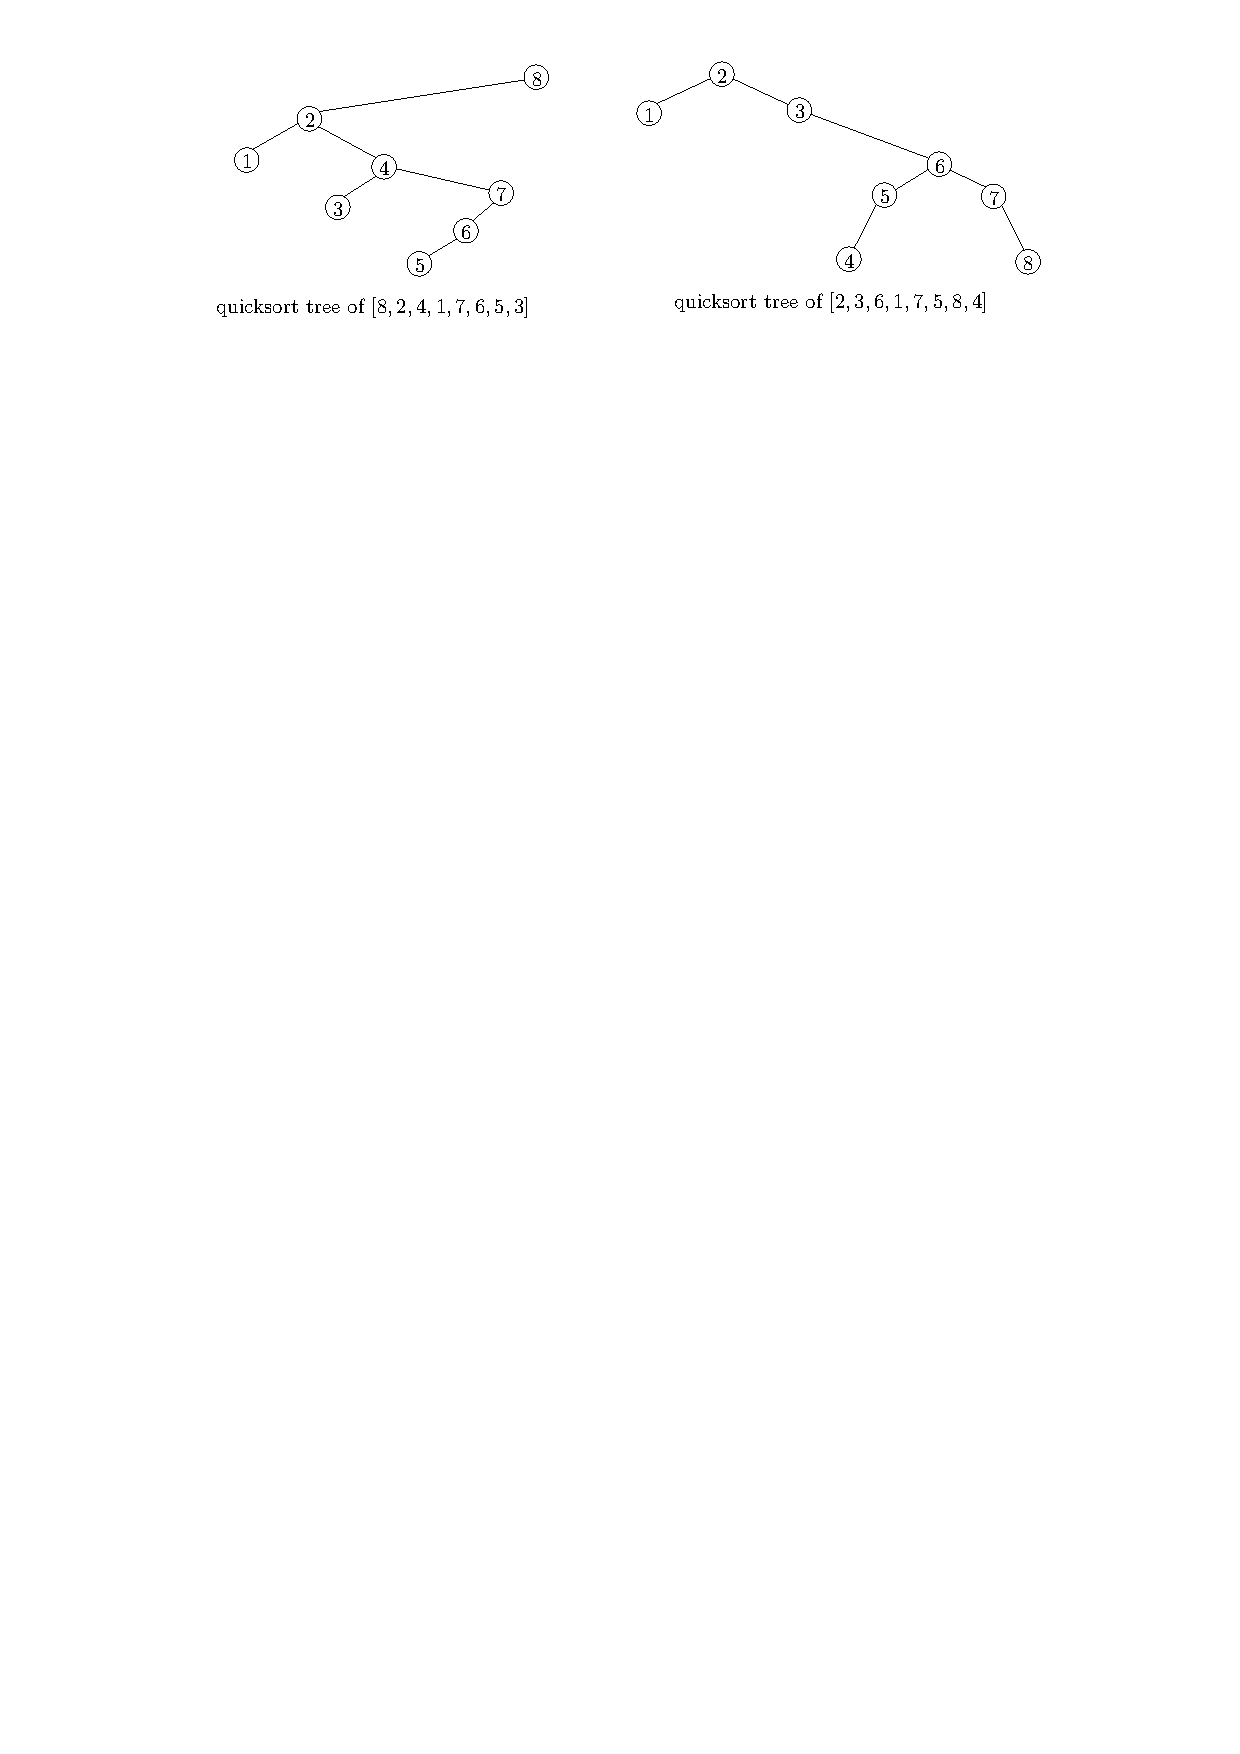
\includegraphics[width=\textwidth]{figures/quicksort-tree.pdf}
\end{center}

We denote a specific list (ordering) by $\pi$ and the tree by $T(\pi)$. $A_{i,j}$ is an indicator
variable which is $1$ if $i$ is an ancestor of $j$ in the tree $T(\pi)$, and $0$ otherwise.
In the lecture, we have derived:
\begin{align*}
	\E[A_{i,j}] & = \frac{1}{|i-j|+1} \\
	\textnormal{ total number of comparisons } & = \sum_{i \ne j} A_{i,j} \ . 
\end{align*}


\begin{exercise}
 Determine the expected number of comparisons made by quicksort. 
 Your final formula must be {\em closed}, meaning it must not contain 
 $\E$, $\prod$, or $\sum$. It may, however, contain $H_n := 1 + \frac{1}{2} + \frac{1}{3} + 
 \dots + \frac{1}{n}$ , the 
 $\nth{n}$ Harmonic number. \textbf{Remark.} This gets a bit tricky, and you will need some
 summation wizardry towards the end.
 \end{exercise}
 

\subsection{Quickselect}

Remember the recursive algorithm \textsc{QuickSelect} from the lecture. I write
it below in pseudocode. In analogy to quicksort we define QuickSelect deterministically
and assume that the input array is random, or has been randomly shuffled before
QuickSelect is called. We assume that $A$ consists of distinct elements and
$1 \leq k \leq |A|$.

\begin{algorithm}
\caption{Select the \nth{$k$} smallest element from a list $A$}
\begin{algorithmic}[1]
\Procedure{QuickSelect}{$X,k$}
  \If{$|X| = 1$}
    \State \Return $X[1]$
  \Else:
  \State $p := X[1]$
  \State $Y:= [ x \in X \ | \ x < p]$
  \State $Z := [ x \in X \ | \ x > p]$
  \If{$|B| = k-1$}
   	\State \Return $p$
  \ElsIf{$|Y| \geq k$}
     	\State \Return $\textsc{QuickSelect}(Y,k)$
  \Else
  	\State Return $\textsc{QuickSelect}(Z, k- |Y| - 1)$
  \EndIf
  \EndIf
\EndProcedure
\end{algorithmic}
\end{algorithm}


Let $C$ be the number of comparison made by $\textsc{QuickSelect}$. In the 
lecture we proved that $\E[C] \leq O(n)$ when we run it on a random input.

\begin{exercise}
	Explain how \textsc{QuickSelect} can be viewed as a ``partial execution'' of quicksort
	with the random pivot selection rule.
	Draw an example quicksort tree and show which part of this tree is visited
	by \text{QuickSelect}.
\end{exercise}


\begin{center}
 	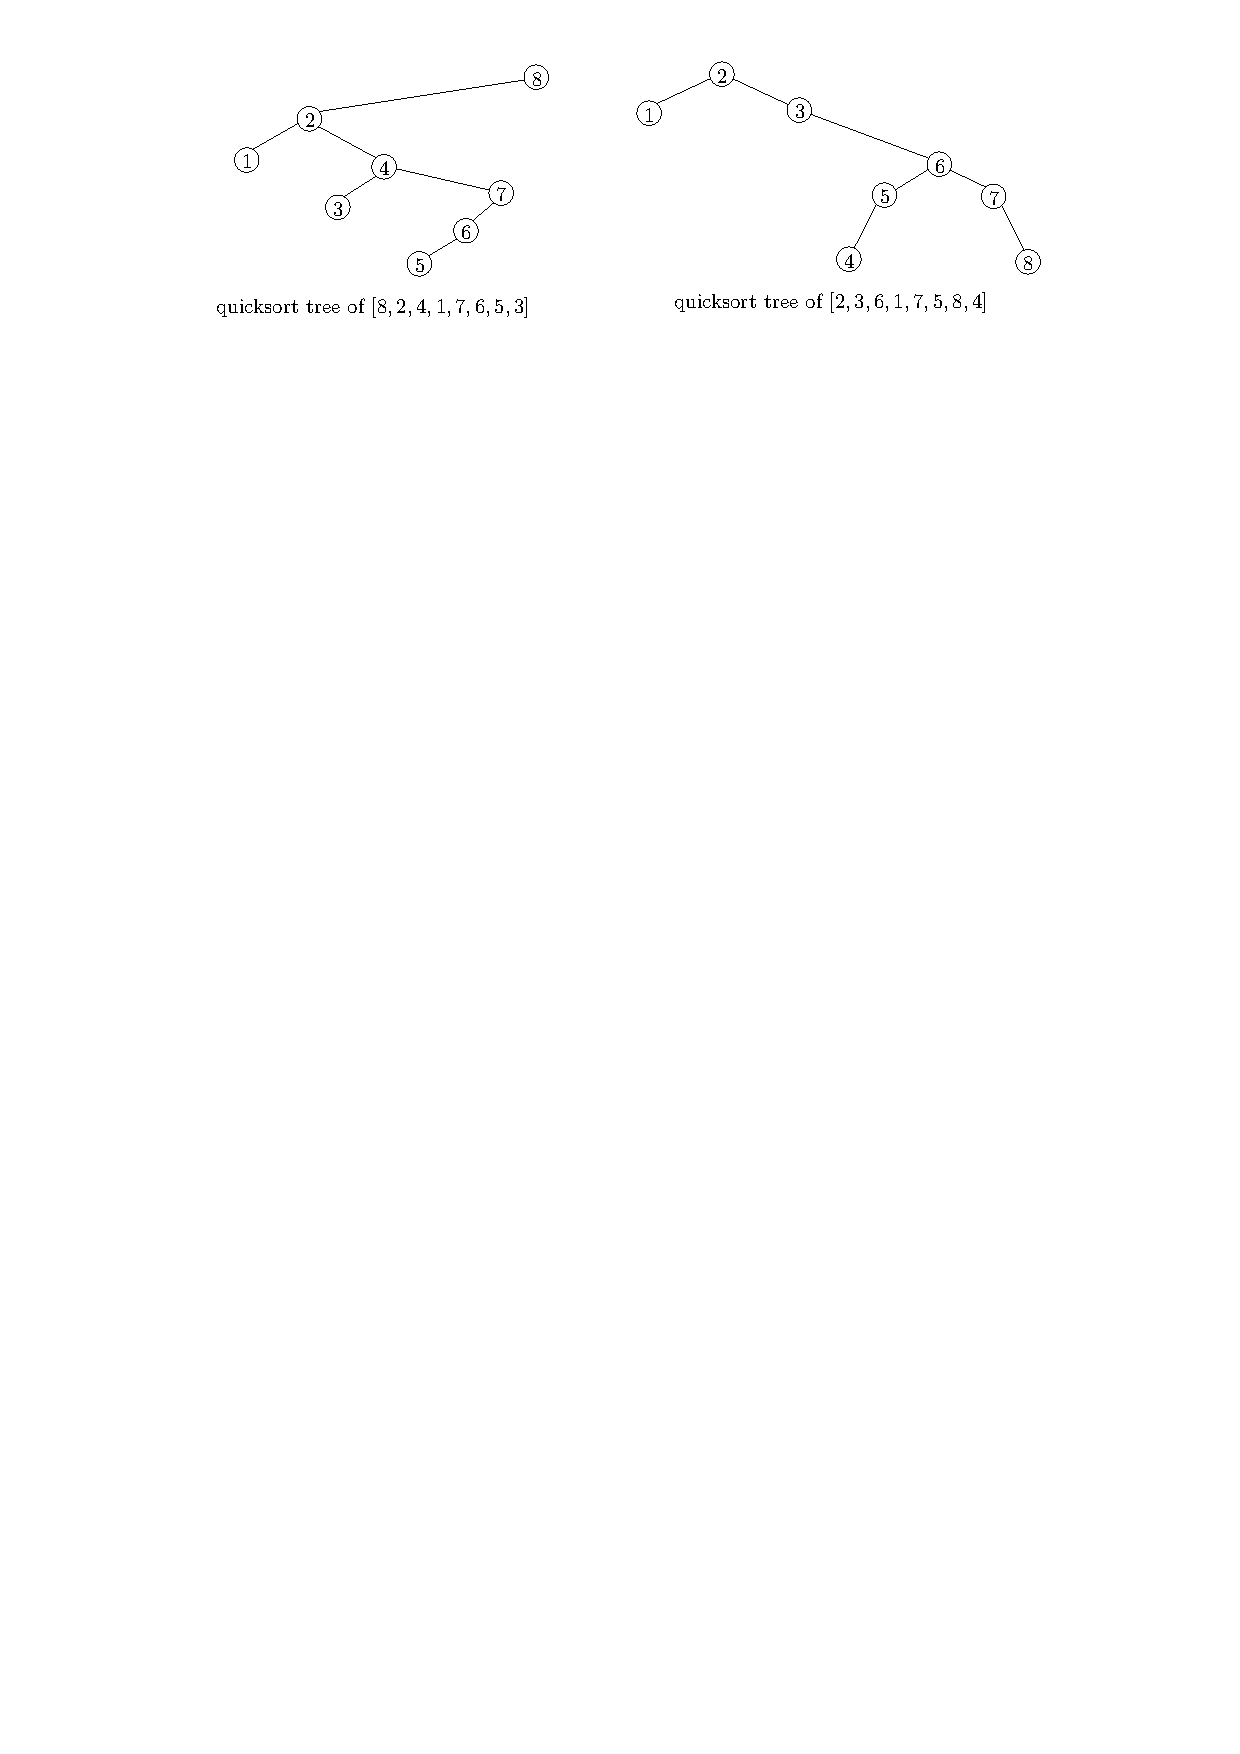
\includegraphics[width=\textwidth]{figures/quicksort-tree.pdf}
\end{center}
\begin{proof}
	For example, if quicksort-tree is left-side tree and k=5, then the visit order of quickselect algorithm is [8, 2, 4, 7, 6, 5]. This is a chain from the root to one of the nodes. Everytime, if the pivot fits the rank we want to find, the result is it. Otherwise, we will recusive the interval fitted the rank what represents the left or right child in quicksort-tree. So, now we get the conclusion: quickselect can be viewed as a "a partial execution" of quicksort with random pivot selection rule.
\end{proof}



Let $B_{i,j,k}$ be an indicator variable which is $1$ if $i$ is a common ancestor
of $j$ and $k$ in the quicksort tree. That is, if both $j$ and $k$ appear in the 
subtree of $T(\pi)$ rooted at $i$.

\begin{exercise}
   What is $\E[B_{i,j,k}]$? Give a succinct formula for this.
\end{exercise}



\begin{exercise}
  Let $C(\pi,k)$ be the number of comparisons made by \textsc{QuickSelect} when given
  $\pi$ as input. Design a formula for $C(\pi,k)$ with the help of the indicator
  variables $A_{i,j}$ and $B_{i,j,k}$ (analogous to the formula 
  $\sum_{i \ne j} A_{i,j}$ for the number of comparisons made by quicksort).
\end{exercise}


\begin{exercise}
   Suppose we use \textsc{QuickSelect} to find the minimum of the array. On expectation,
   how many comparisons will it make? Give an answer that is exact up to additive terms 
   of order $o(n)$.
     You can use the fact that $H_k := 1 + \frac{1}{2} + \frac{1}{3} + \cdots  + \frac{1}{n} = \ln(n) + o(1)$.
\end{exercise}

\begin{exercise}
  Derive a formula for $\E_{\pi} [C(\pi,k)]$, up to additive terms of order $o(n)$.
  You might want to introduce $\kappa := k/n$.
\end{exercise}


\end{document}

\subsection{Other Recurrences}

Suppose we are given the recurrence
\begin{align*}
T(n) := \begin{cases}
0 &  \text{if } n \leq 1 \ , \\
 2T(n/2) + n & \text{else.}
\end{cases} \ .
\end{align*}
By looking at the recursion tree, where were able to show that $T(n) \leq n \log(n)$, 
and in fact $T(n) = n \log(n)$ if $n$ is a power of $2$.

\begin{exercise}
   Extend your proof from the previous exercise. Suppose we are given numbers
   $p_1,\dots, p_k \in (0,1)$ such that $p_1 + \cdots + p_k = 1$. Let
\begin{align*}
T(n) := \begin{cases}
0 &  \text{if } n=1 \ , \\
 n +  \sum_{i=1}^k T(p_i n)  & \text{else.}
\end{cases} \ .
\end{align*}  
It is easy to see that $T(n) \in \Theta( n \log n)$, too. However, I want you to determine
the constant factor. That is, determine a number $\gamma$ such that $T(n) = \gamma n \log n + 
o(n \log n)$. \textbf{Remark.} For this, looking at the recursion tree level by level might not be enough. 
You may have to prove it by induction and see for which value of $\gamma$ it ``goes through''.
\end{exercise}



\end{document}